\documentclass{article}

\usepackage{graphicx}
\usepackage{tikz}
\usepackage{tikzsymbols}
\usetikzlibrary{calc,patterns,shapes.geometric}
\pagestyle{empty}
\usepackage[margin=0pt]{geometry}
\geometry{papersize={14in,12in}}

\def\centerarc[#1](#2)(#3:#4:#5){\draw[#1] ($(#2)+({#5*cos(#3)},{#5*sin(#3)})$) arc (#3:#4:#5);}

\begin{document}
	\begin{figure}
		\centering
		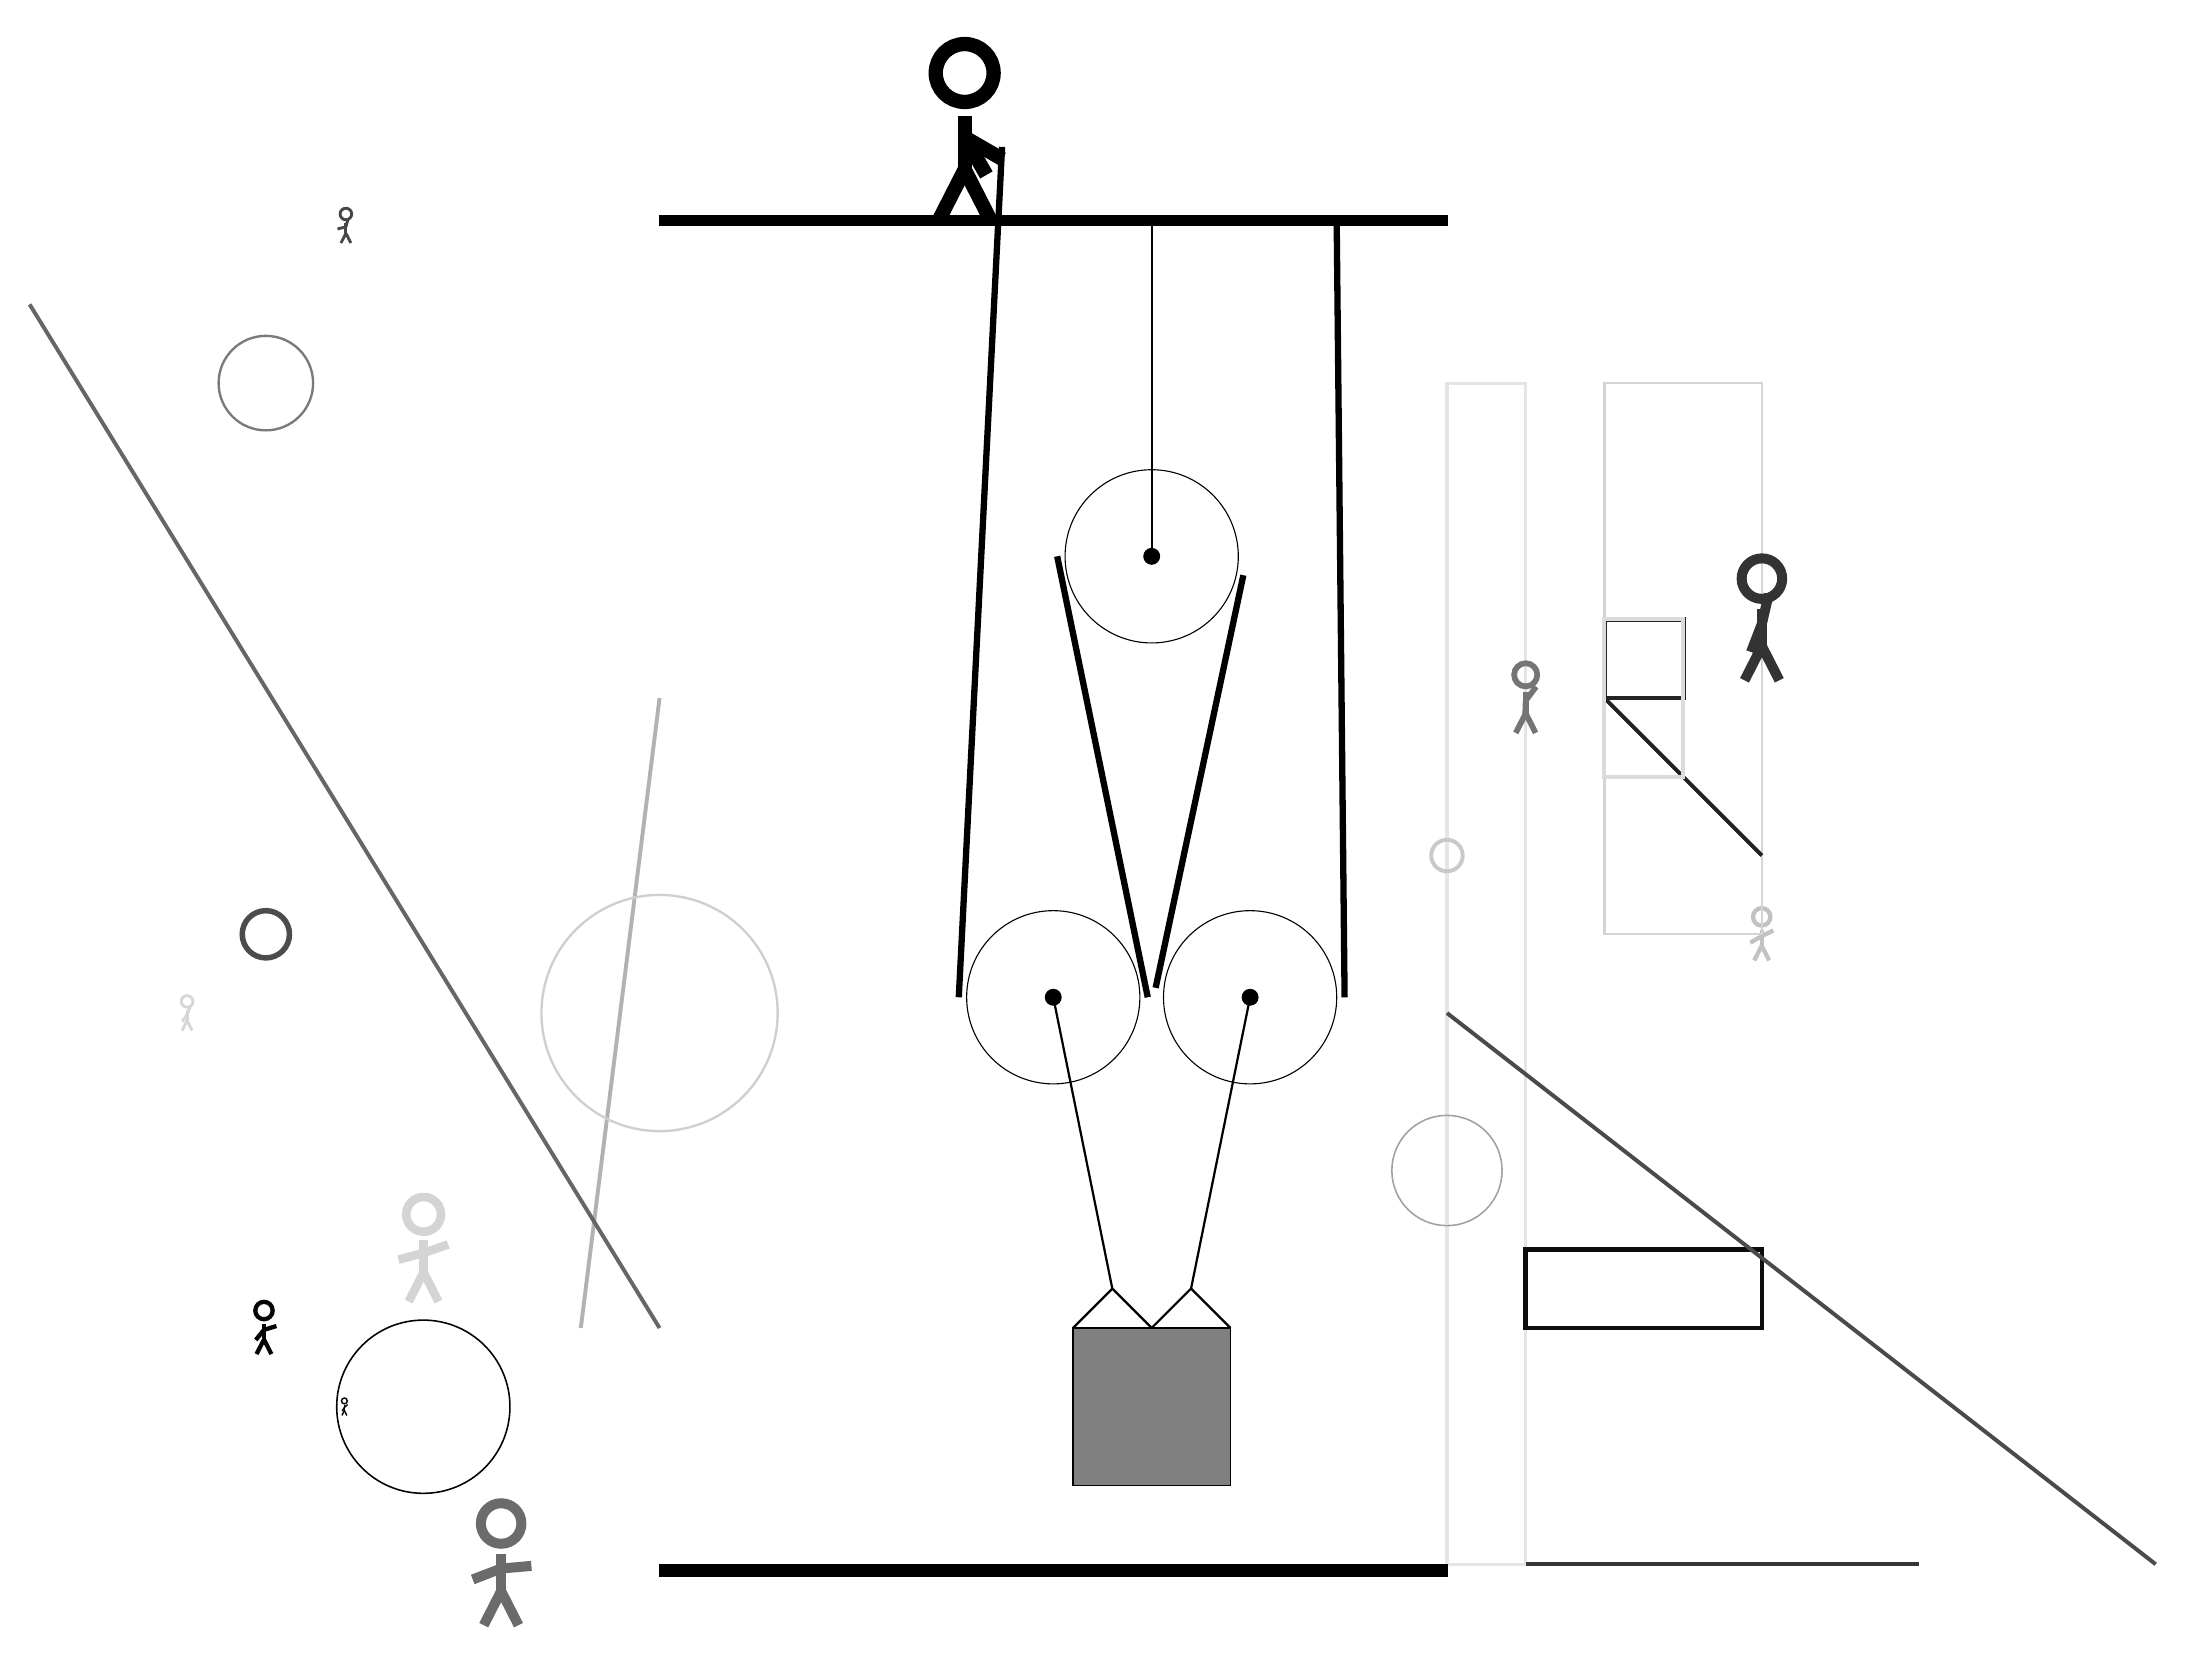
\begin{tikzpicture}
			%%%%% START %%%%%
			
			\draw[fill=black] (-4, 14) rectangle (6, 14.125);
			
			\draw (1, 4.2) circle (1.1);
			\draw[fill=black] (1, 4.2) circle (0.1);
			
			\draw (2.25, 9.8) circle (1.1);
			\draw[fill=black] (2.25, 9.8) circle (0.1);
			\draw[thick] (2.25, 9.8) -- (2.25, 14);
			
			\draw (3.5, 4.2) circle (1.1);
			\draw[fill=black] (3.5, 4.2) circle (0.1);
			
			\draw[thick] (3.5, 4.2) -- (2.75, 0.5);
			\draw[thick] (1, 4.2) -- (1.75, 0.5);
			\draw[thick]  (1.25, 0) -- (1.75, 0.5) -- (2.25, 0);
			\draw[thick]  (2.25, 0) -- (2.75, 0.5) -- (3.25, 0);
			\draw[fill=black!50] (1.25, 0) rectangle (3.25, -2);
			
			\draw[line width=0.8mm] (0.35, 15) --  (-0.2, 4.2);
			\centerarc[line width=0.8mm](1, 4.2)(180:360:1.2000000000000002);
			\draw[line width=0.8mm] (2.2, 4.2) -- (1.05, 9.8);
			\centerarc[line width=0.8mm](2.25, 9.8)(-20:180:1.2000000000000002);
			\draw[line width=0.8mm](3.414, 9.56) -- (2.3, 4.32);
			\centerarc[line width=0.8mm](3.5, 4.2)(160:360:1.2000000000000002);
			\draw[line width=0.8mm](4.7, 4.2) -- (4.6, 14);
			
			\node[line width=0.4mm, color=black!24] at (10, 5) {\Strichmaxerl[3][30][26]};
			
			\draw [line width=0.3mm, color=black!52](-9, 12) circle (0.6);
			\draw[line width=0.4mm, color=black!10] (7, 12) rectangle (6, -3);
			\draw[line width=0.3mm, color=black!17] (8, 5) rectangle (10, 12);
			\draw[line width=0.5mm, color=black!87](10, 6) -- (8, 8);
			
			\node[line width=0.7mm, color=black!72] at (-8, 14) {\Strichmaxerl[2][14][75]};
			\draw [line width=0.5mm, color=black!21](6, 6) circle (0.2);
			\node[line width=0.3mm, color=black!98] at (-9, 0) {\Strichmaxerl[3][51][17]};
			\draw[line width=0.5mm, color=black!30](-4, 8) -- (-5, 0);
			\draw[line width=0.6mm, color=black!95] (7, 0) rectangle (10, 1);
			\node[line width=0.5mm, color=black!17] at (-7, 1) {\Strichmaxerl[6][15][19]};
			\node[line width=0.4mm, color=black!54] at (7, 8) {\Strichmaxerl[4][88][53]};
			\draw[line width=0.5mm, color=black!71](6, 4) -- (15, -3);
			
			\node[line width=0.2mm, color=black!58] at (-6, -3) {\Strichmaxerl[7][21][5]};
			\draw[line width=0.6mm, color=black!86] (8, 8) rectangle (9, 9);
			\node[line width=0.5mm, color=black!97] at (-8, -1) {\Strichmaxerl[1][60][40]};
			
			\draw[line width=0.5mm, color=black!60](-4, 0) -- (-12, 13);
			\draw[line width=0.5mm, color=black!14] (8, 7) rectangle (9, 9);
			\draw[line width=0.5mm, color=black!79](7, -3) -- (12, -3);
			\draw [line width=0.2mm, color=black!99](-7, -1) circle (1.1);
			\draw [line width=0.7mm, color=black!70](-9, 5) circle (0.3);
			
			\draw [line width=0.3mm, color=black!19](-4, 4) circle (1.5);
			\node[line width=0.2mm, color=black!16] at (-10, 4) {\Strichmaxerl[2][57][67]};
			\draw [line width=0.2mm, color=black!37](6, 2) circle (0.7);
			\node[line width=0.3mm, color=black!80] at (10, 9) {\Strichmaxerl[7][69][77]};
			
			\node at (-0.07, 15.2) {\Strichmaxerl[10][120][-30]};
			
			\draw[fill=black] (-4, -3) rectangle (6, -3.15);
			
			%%%%% END %%%%%
		\end{tikzpicture}
	\end{figure}	
\end{document}